% !TeX spellcheck = en_GB
\documentclass[a4paper,doc,floatsintext,natbib,10pt]{apa6}
\title{Flow experiences across longitudinal visuomotor skill acquisition reflect spontaneous blink rate variation}
\shorttitle{Flow Experience and spontaneous blink rate}

% FIXME - data and analysis code in a repository

% insert here the call for the packages your document requires
% \usepackage{graphics}
\graphicspath{{./Figures/}}
% \usepackage[latin1]{inputenc}
\usepackage{amsmath}
\usepackage{amsfonts}
\usepackage{amssymb}
\usepackage{url}
\usepackage{xspace}
\usepackage{textcomp}
\usepackage{xcolor}
\usepackage{varwidth}
\usepackage{todonotes}
\usepackage{caption}
\usepackage[normalem]{ulem}
\usepackage[auth-lg]{authblk}
\usepackage{xcolor}
\usepackage{varwidth}

\newcommand{\hl}{\textcolor{red!80}}
\newcommand{\CCS}{\textsf{CogCarSim}\xspace}
\newcommand{\nicewidth}{0.75\textwidth}
\newcommand{\tapprx}{\raisebox{0.4ex}{\texttildelow}}

\author[1,2 *]{Benjamin Ultan Cowley}
\author[1,5]{Jussi Palom\"{a}ki}
\author[1,3]{Tuisku Tammi}
\author[1,3]{Roosa Frantsi}
\author[1,4]{Ville-Pekka Inkil\"{a}}
\author[1]{Noora Lehtonen}
\author[1]{Pasi P\"{o}l\"{o}nen}
\author[1]{Juha Veps\"{a}l\"{a}inen}
\author[1,3,5]{Otto Lappi}

\affil[1]{Cognitive Science, Department of Digital Humanities, University of Helsinki, Helsinki, Finland}
\affil[2]{Cognitive Brain Research Unit, Department of Psychology and Logopedics, University of Helsinki, Helsinki, Finland}
\affil[3]{TRUlab, University of Helsinki, Helsinki, Finland}
\affil[4]{Digitalization, Finnish Institute of Occupational Health, Helsinki, Finland}
\affil[5]{Helsinki Centre for Digital Humanities (HELDIG)}


\affiliation{* ben.cowley@helsinki.fi}

\abstract{Flow is a state of `optimal experience' that arises when skill and task demands match. Flow has been well studied in psychology using a range of self-report and experimental methods; with most research typically focusing on how Flow is elicited by a particular task. Here, we focus on how the experience of Flow changes during task skill development. We present a longitudinal experimental study of learning, wherein participants (N = 9) play a novel steering-game task designed to elicit Flow by matching skill and demand, and providing clear goals and feedback. Experimental design involves extensive in-depth measurement of behaviour, physiology, and Flow self-reports over two weeks of 40 game trials in eight sessions. Behavioural results are both strikingly similar and strong within each participant. We find that the game induces a near-constant state of elevated Flow. We further find that the variation in Flow across all trials is less affected by overall performance improvement than by deviation of performance from the expected value predicted by a power law model of learning. Finally, concurrent measurement of physiology shows that spontaneous blink rate, a putative index of striatal dopamine, relates to the individual rate of learning, and that this relationship is moderated by Flow.\\

\textbf{Keywords:} Flow, Skill Acquisition, spontaneous blink rate, Visuomotor performance, Steering, high performance cognition
}

\begin{document}
\maketitle


\section*{Introduction}

In many fields of human endeavour - such as music, art and sports - the skilful performance of a demanding task can elicit a state of `optimal experience' called Flow \citep{Csikszentmihalyi1975}. The conditions for Flow are: {\sf C1} challenges match skill in a demanding task; {\sf C2} clear and personally significant goals; and {\sf C3} unambiguous feedback on goal achievement. When these conditions are met, an individual may enter a mode of high performance characterized by several self-reported features: {\sf F1} total focus in the present moment, and concentration on what one is doing; {\sf F2} merging of action and awareness (being `one' with the task); {\sf F3} loss of reflective self-consciousness or a sense of effortlessness and automaticity; {\sf F4} a sense of personal control and confidence in one's skill; {\sf F5} positive affect, or an experience of the activity as highly enjoyable and intrinsically rewarding; {\sf F6} a distortion of temporal experience (time may seem to go slower or faster than normal) \citep{Nakamura2002,Engeser2012intro,Keller2012}. Flow has an autotelic quality, i.e. people want to do Flow-producing activities for their own sake regardless of external reward.

The antecedent conditions ({\sf C1-3}) and phenomenological features ({\sf F1-6}) of Flow have been investigated for several decades, mainly using analysis of self-report data from participants engaging in natural everyday or expert performance \citep{Csikszentmihalyi1971,Moneta2012}. Despite this, debate continues around the precise definition of conditions, especially {\sf C1}. There are multiple models of Flow which have different interpretations of the skill-challenge balance required for Flow, from which different predictions can be derived for how Flow should change when skill and challenge themselves change during learning. The original channel model \citep{Csikszentmihalyi1975} assumed levels of challenge and skill can vary independently from low to high, and assumed Flow can be induced when skill and challenge match at any level, giving the Flow `channel'.

The now-classic octant/quadrant models \citep{Massimini1988} instead suggested Flow only happens above a threshold level of skill and challenge. Too-low perceived task demand would not elicit Flow, even when matching skill. This model has been criticized on the grounds that it remains unclear how the reference level is determined: does challenge need to exceed the challenge of most typical everyday tasks? Does the task need to be particularly challenging for the individual, challenging relative to typical skills of a reference population, or in comparison to some absolute level of physical effort or information processing complexity? Or is challenge task-specific? In which case, what happens during task learning? Does the reference level need to be recalibrated to suit (presumably) increased levels of skill and challenge? For further discussion and critical examination of these models see \cite{Moneta2012,Keller2012}.

Recently \citet[pp-56]{Keller2012} proposed the Flow intensity model, using perceived challenge--skill balance and subjective value of the task as dimensions of Flow-eliciting conditions. This model has no reference levels at all, thus handling the ambiguity of the reference level concept and also their argument that level might not be empirically determinable for researchers, or even psychologically available to performing individuals. But here, the direction of a challenge--skill imbalance has no effect: only the absolute magnitude counts.

Thus, the state of the art is unclear on whether reference levels of challenge and/or skill govern the emergence of Flow. If they do, it is unclear whether the levels are defined relative to a given task or task episode (in which case should the level change with skill acquisition); or are they defined relative to other tasks (in which case, should the comparison of task demand be understood relative to the skill sets of the individual, a reference population, or an absolute standard). Also unclear is importance of direction in skill--challenge ratio, i.e. whether it makes a difference that skills exceed challenge or challenge exceed skill. Finally, these models capture a static snapshot of Flow, so Flow research must still deal with \textit{learning} that increases skill and the effects thereof on {\sf C1}, skill-challenge balance condition.

%anticipate MAIN RESULT and its IMPLICATIONS here
The matter is of importance because understanding how the Flow conditions behave across different levels of skill is relevant to any field interested in the development of performance (in e.g. development of coaching practices or concentration techniques in sport \citep{Jackson1996}). Also, an understanding of the specific mechanisms that mediate Flow and learning could be significant for enhancing enjoyment or performance in many tasks (e.g. through better design of recreational tasks such as games \citep{Chen2007}). However, these aims call for studies of Flow as elicited in different phases of learning, with a more controlled and quantitative approach; i.e. using approaches from experimental psychology \citep{Harris2017,Keller2008}, and psychophysiology \citep{Peifer2012,Peifer2014,Wolf2015,Harmat2015,Labonte-LeMoyne2016}.

This paper reports an experimental skill-acquisition study on the connections between performance, psychophysiology and the self-reported phenomenology of Flow. We introduce a novel, demanding visuomotor task. With a longitudinal design, we are afforded more power to examine the connections of Flow and performance within- and between-subjects.

To anticipate the findings, our task succeeds in eliciting an elevated level of Flow across all self-reports. Yet when we examine Flow with fine granularity, we see that variation in Flow responses relates less to overall performance improvement, than it does to deviation of performance from the expected value predicted by a power law model of learning, with higher performance associated with higher Flow and lower performance with lower Flow. These results show that: 1. Contrary to the \cite{Keller2012} model the direction of challenge-skill deviation cannot be ignored; 2. If a reference level is important (as the octant model requires), it is so on a trial-wise scale. I.e. the reference level is task-specific and is continually adjusted during skill acquisition, following in step with the individual's own learning curve.

Our study highlights a need for models of Flow to be developed in a way that better captures Flow dynamics, over the range of skill acquisition from novice to expert, than the state-like models of the phenomenal psychology tradition \citep{Moneta2012}.

\paragraph{Protocol and Research Questions}

Participants learned to play a custom-made high-speed steering game (Fig.~\ref{fig:cogcarsim}, for game video see \url{https://doi.org/10.6084/m9.figshare.7269395.v1}). The game was specifically designed to elicit Flow through balancing task demand with the skill level of the participant, and providing clear immediate feedback. The aim in the game was to steer a blue cube through a course with randomly placed red obstacles at the highest possible speed. The cube started each game at a fixed forward velocity, which increased at a constant rate. The lateral position of the cube was controlled by the steering wheel. Collision with obstacles reduced speed by a fixed amount, also indicated by a flashing of the screen (see Methods for units).

This design, inspired by psychophysical staircase methods \citep{Cornsweet1962}, ensured constant match between skill and demand at the participant's level of performance. The performance was measured by duration of the trial (shorter duration = faster average speed = better), displayed as a time score at the end of each trial.

\begin{figure*}[!ht]
	\centering
	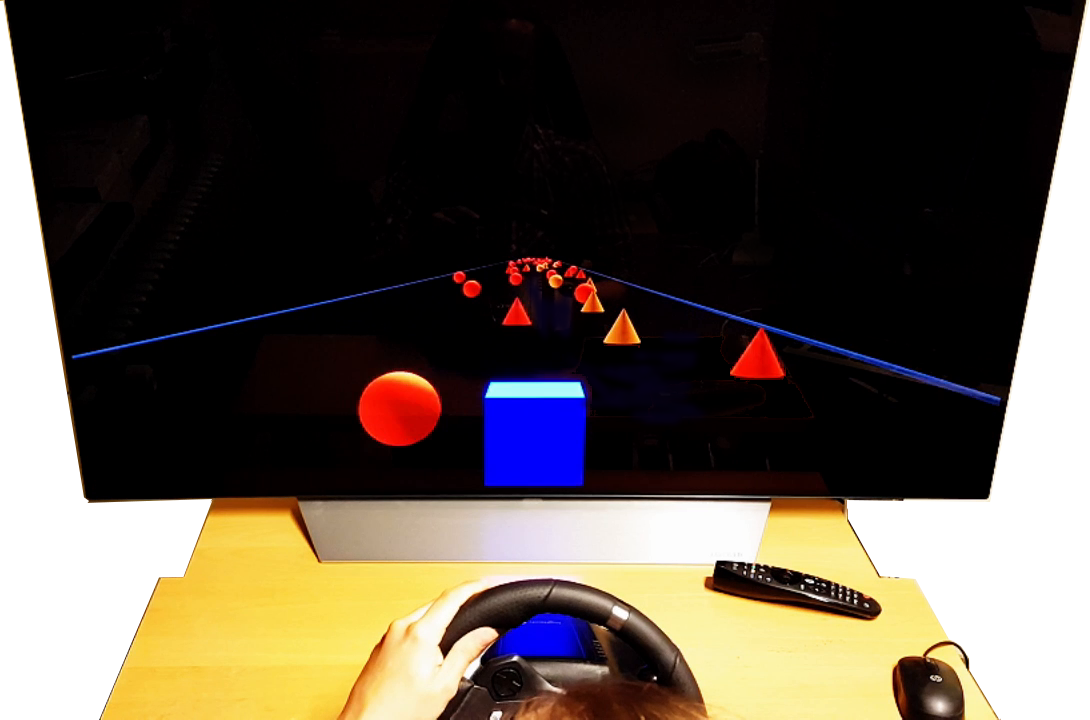
\includegraphics[width=\nicewidth]{Screenshot_cogcarsim}
	\caption{The high-speed steering task. The participant steers the blue cube to avoid conical/spherical obstacles on the track, which is bounded to each side by dark blue parallel lines. The game was designed to continually adapt the difficulty level (speed) to the participant's skill (obstacle collisions). Such balance is considered one of the key antecedents of Flow.}
	\label{fig:cogcarsim}
\end{figure*}

Participants played the game for forty trials across eight sessions, over a period of 2-3 weeks, which was sufficient to achieve good proficiency in this task with no ceiling effect. The 10 item Flow Short Scale \citep{Engeser2008} was filled after each trial to probe self-reported Flow in the task. Physiological data were recorded, during task and five minutes of baseline, in sessions one and five-to-eight.

This design allowed us to explore the following Research Questions:
\begin{enumerate}
	\item RQ1. Are there identifiable physiological markers of Flow and/or physiological measures that are predictive of task performance? Specifically, given its putative association with striatal dopamine \citep{Slagter2012}, spontaneous eye blink rate (sEBR) was of interest in our reinforcement-based learning task (positive reinforcement from increase in speed, negative reinforcement from collisions). \hl{Other measures were collected as well, but will be analysed and reported elsewhere; here we focus on the sEBR results.}

	\item RQ2. blink rate and Flow components?

	\item RQ3. performance, blink rate, and Flow components?

\end{enumerate}


%%%%%%%%%%%%%%%%%%%%%%%%%%%%%%%%%%%%%%%%%%%%%%%%%%%%%%%%%%%%%%%%%%%%%%%%%%%%%%%%
%%%%%%%%%%%%%%%%%%%%%%%%%%%%%%%%%%%%%%%%%%%%%%%%%%%%%%%%%%%%%%%%%%%%%%%%%%%%%%%%
%%%%%%%%%%%%%%%%%%%%%%%%%%    METHODS    %%%%%%%%%%%%%%%%%%%%%%%%%%%%%%%%%%%%%%%
\section*{Methods}
% !TEX root = main.tex

\subsection*{Participants}
A convenience sample (N=9, 6 males, 3 females) was recruited via student mailing lists at the University of Helsinki. The participants were between 22-38 years of age (mean 27, SD 3) with normal or corrected-to-normal visual acuity and no history of neurological or psychiatric disease.

\begin{table}[ht]
\centering
\caption{\label{tab:Participants}Participant background information.}
\begin{tabular}{llllll}
\hline
Participant & Gender & Age & Driving license & Driving experience (km) & Gaming experience \\
\hline
1 & M & 27 & yes & 1,000-10,000 & At least one hour a week \\
2 & M & 23 & yes & 10,000-30,000 & At least one hour a week \\
3 & F & 23 & no & 0-1,000 & None or very little \\
4 & F & 28 & yes & 0-1,000 & At least one hour a week \\
5 & M & 27 & yes & 30,000-100,000 & At least one hour a week \\
6 & M & 22 & yes & 30,000-100,000 & 1-3 hours a month \\
7 & F & 31 & yes & 10,000-30,000 & None or very little \\
8 & M & 38 & yes & 100,000+ & 1-3 hours a month \\
9 & M & 25 & yes & 10,000-30,000 & At least one hour a week \\
\hline
\end{tabular}
\end{table}

Eight of the participants had a driving license; two participants reported $<$10,000 km lifetime kilometrage, three participants 10,000-30,000 km, two 30,000-100,000 km, and one participant $>$100,000 km. Two had no or very little previous gaming experience, two participants played 1-3 hours a month, and five participants stated they play over one hour a week.

All participants were naive about the specific hypotheses and purpose of the study, other than that the time of recruiting they were informed that the experiment was about game experience and learning. Participants were given 11 cultural vouchers (1 voucher is worth 5 euro) in compensation for their time. They were told that they would get 9 vouchers for participating in all sessions and 2 extra vouchers if they improved their performance in the game. The criteria for sufficient improvement were not stated explicitly, and in fact all participants were given the two extra vouchers.

Participants were briefed and provided written informed consent before entering the study, and were aware of their legal rights. The study followed guidelines of the Declaration of Helsinki and was approved by the University of Helsinki Ethical review board in humanities and social and behavioural sciences (statement 31/2017; study title MulSimCoLab).

\subsection*{Design}
The experiment was divided into eight sessions, on eight different days over a period of 2-3 weeks scheduled at each participant's convenience. In each session, the participant played five trials of the driving game, each trial lasting 2-4 min depending on their performance, for approximately 15 min of driving time per session. The judgement of how much total playtime (here, \tapprx2hrs) would be sufficient to develop good task proficiency was based on extensive informal piloting, including prior observations with other convenience samples.

After each trial, the participant was shown the trial duration and the number of collisions, after which they filled in a self-report questionnaire (FSS). In sessions 1 and 5-8 (lasting approx. an hour), physiological signals were measured in a 5 minutes baseline recording before playing, and during gameplay. In sessions 2-4 (lasting 20 to 30 minutes), no physiological measurements were taken.

\begin{figure*}[!ht]
\centering
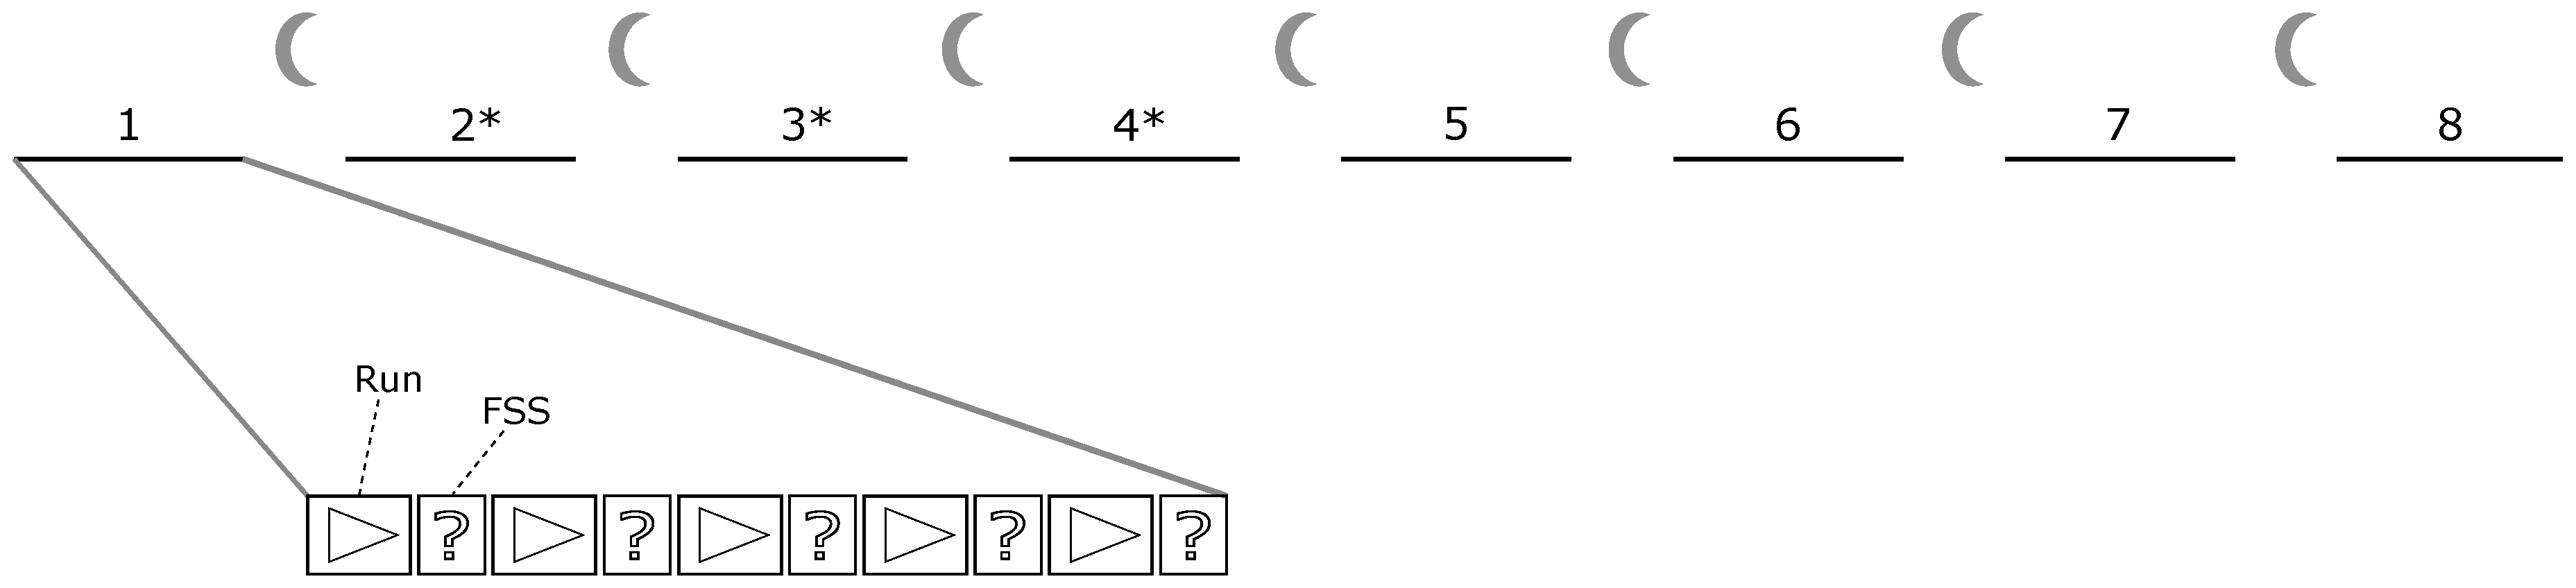
\includegraphics[width=\nicewidth]{design1}
\caption{The game was played in eight sessions on eight different days. In sessions 1 and 5--8, physiological signals were recorded during task performance; in sessions 2-4(*) no physiology was recorded. Each session consisted of five trials (2 to 4 min) followed by a self-report questionnaire (FSS, Flow Short Scale) about the latest trial.}
\label{fig:design}
\end{figure*}

\subsection*{Materials}
\paragraph{Game} The experimental task was a custom-made high-speed steering game {\it CogCarSim} designed specifically for the study of Flow and coded in Python. The game code as used herein is permanently available under open source licence at \url{https://doi.org/10.6084/m9.figshare.7269467}.

The participant steered a cube `avatar' moving forward along a straight track bounded by edges that could not be crossed. The cube's side length was 2 units, and the track was 25 units wide.  The horizontal field of view angle of the virtual camera was 60 degrees and vertical 32 degrees. The camera was positioned behind the cube at 4 units height, pointing forward along the track.

Stationary obstacles (red cones, red or yellow spheres with a height/diameter of 2 units) on the track had to be avoided. For each trial, a total of 2,000 obstacles were placed randomly on the track, with placement constrained to always allow a path through. Track length varied between 24196.4 and 24199.7 units (mean 24197.8, sd 0.8). The speed of the cube was initially set to 1.6 units per step (96 units per second); increased at a constant rate (0.0012 units/step at every step); and slowed down if obstacles were hit (0.102 units/step at each collision). When a collision caused a speed drop, the screen flashed to indicate a collision; there followed an immunity period of 100 steps during which additional collisions did not cause further speed drops. Participants could only affect speed indirectly, by avoiding collisions.  Participants were instructed to avoid as many obstacles they could in order to complete the trial as fast as possible.

The game had maximally simple one degree-of-freedom linear and holonomic dynamics: the horizontal position of the cube was directly proportional to steering wheel angle. Extensive self-piloting was done to adjust the graphics, e.g. virtual eye height; plus starting and increment speeds, rate of change of speed during collisions, and steering wheel sensitivity (steering ratio and damping).

The participants started each trial by pressing a button on the steering wheel when they felt ready. At the end of each trial, the elapsed time and number of collisions were displayed, along with a high score of the participant's ten best trials so far.

Data collected by CogCarSim included the positions, shape, and colour of obstacles on the track; trial-level aggregated performance data (trial duration, number of collisions, average velocity); and within-trial time series data (steering wheel and cube position, speed, registered collisions).

\paragraph{Equipment} The game was run on a Corsair Anne Bonny with Intel i7 7700k processor and an Nvidia GTX 1080 graphics card, running Windows 10. Eye-tracking and physiological signals were collected and stored on an Asus UX303L laptop with Debian GNU/Linux 9 OS.

The participant was seated in a Playseat Evolution Alcantara playseat (Playseats B.V., The Netherlands) aligned with the mid point of the 55" display screen (LG 55UF85). The screen resolution was 1920 x 1080 pixels, the frame rate was 60 and the refresh rate 60 Hz. The viewing distance was adjusted for each participant (so that they could place their hands on the steering wheel comfortably) and was approximately between 90 and 120 cm from the eye to the screen. The game was controlled with a Logitech G920 Driving Force steering wheel (Logitech, Fremont, CA). Steering wheel settings in Logitech Gaming Software 8.96.88 were: sensitivity 100 percent, centering spring strength 4 percent, and wheel operating range 900 degrees.

Eye movements (not reported here) were measured using Pupil Labs Binocular 120 Hz eye tracker (Pupil Labs UG haftungsbeschränkt, Berlin, Germany), stabilised with a custom-built headband. Pupil Capture software was used to collect the data from the pupil hardware. Gaze direction was calibrated using ten markers on the display, a minimum of three times during the session. Additional calibrations were done if needed. Eye movement signal was recorded at 60 Hz.

% For electrodermal activity (EDA, not reported here), Ag-AgCl electrodes with 0.5\% saline paste were attached to the medial side of the left foot with adhesive skin tape and gauze. The plantar site was used instead of the palmar site to minimise artefacts resulting from the use of the steering wheel, as per guidelines by \cite{boucs12}. Blood volume pulse (BVP) was measured using a pulse oximeter sensor attached to the left index toe of each participant. EDA and BVP were recorded at 128 Hz sampling rate using NeXus-10 (Mind Media B.V, Roermond-Herten, The Netherlands) connected to a laptop via bluetooth. The data was recorded using Trusas signal acquisition software, available open access at \url{https://github.com/jampekka/trusas-nexus}.

\paragraph{Flow Short Scale} To measure self-reported Flow, participants were asked to fill in the Flow Short Scale (FSS) after each trial \citep{Rheinberg2003,Engeser2008}. FSS has 10 core items which load the subfactors {\it fluency of performance} (6 items) and {\it absorption by activity} (4 items); plus 3 items for {\it perceived importance}. The response format of FSS is a 7-point Likert scale ranging from {\it Not at all} to {\it Very much}. Higher scores on the scales indicate higher experienced Flow and perceived importance. Example items include ``My thoughts/activities run fluidly and smoothly'' ({\it fluency of performance}), ``I do not notice time passing'' ({\it absorption by activity}), and ``I must not make any mistakes here'' ({\it perceived importance}). See Supplementary Information for full English text and Finnish translation.

Cronbach's alpha for a 10-item scale including the {\it fluency of performance} and {\it absorption by activity} items was .92; Cronbach's alpha was .87 for the 13-item FSS scale including {\it perceived importance} \citep{Rheinberg2003}. FSS authors \citep{Rheinberg2003} suggest using the 10-item scale (excluding {\it perceived importance} subfactor) as a measure of experienced Flow. For our data also, Cronbach's alpha was higher for the core 10- than for 13-item scale. Thus, the Flow scale used in our analyses was formed by averaging the items in the {\it fluency of performance} and {\it absorption by activity} subfactors. The {\it perceived importance} subfactor was used separately in some analyses (see Results).

% (+3 additional items)
In addition to the 13 main items asked after every trial, participants were asked at the end of every session to report 3 more items measuring the fit of skills and demands of the task  \citep{Rheinberg2003}. These items also had 7-point scales, e.g.: ``For me personally, the current demands are... (too low -- -- just right -- -- too high)''.

There was no Finnish translation of the scale available, so it was translated into Finnish by the authors. Two of the authors (native speakers of Finnish, no formal qualifications for English-Finnish translation) first made translations independently; these translations were compared and revised, then reviewed by other Finnish-native authors, and revised.

\subsection*{Procedure}
After recruiting, participants selected eight suitable dates within a three-week period. All sessions took place between 8 a.m. and 7 p.m. at Traffic Research Unit, Department of Digital Humanities, University of Helsinki. In the first session, participants were informed about the procedure of the study and asked to fill in a background information questionnaire, including information on health, driving experience and gaming experience, and an informed consent form.

The sessions were managed by two research assistants at a time, who observed the measurement, out of participants' line of sight behind a partition wall, and took notes about possible confounding factors and problems within the session. In the beginning of each session participants filled in a session-wise questionnaire on the use of contact lenses, restedness, and medication, caffeine, and nicotine intake.

In sessions 2 to 4, participants played five trials straight after filling in the session-wise questionnaire. The FSS was filled after each trial. In sessions with physiological measurements (1 and 5 to 8), participants were dressed in physiological sensors and an eye-tracking headset, seated in the driving seat in quiet, low-light conditions for baseline measurement. They were asked to sit still for five minutes, looking at a dark blue screen, while baseline was recorded. After baseline recording, participants played five game trials, filling FSS after each trial. At the end of Session 8, the participants were debriefed and given the reward of culture vouchers.

\subsection*{Signal preprocessing and analysis}
Eye blinks were counted manually from the eye tracking videos recorded during baseline period of sessions 1 and 5--8. Three-minute periods were considered sufficient for this purpose, thus the first and last minute from each five-minute recording were omitted to obtain the most stable period of baseline. Four measurements (out of 40) were excluded due to measurement problems.

All fast and simultaneous movements of both eyelids were counted as blinks (even if the eyelid did not fully close). To ensure reliable blink identification, two of the authors independently counted the number of blinks in sessions 1, 6 and 8, and inter-rater reliability of the counts was calculated as 98.7\% (see below). We considered this high enough to have blinks in remaining sessions 5 and 7 counted by only one experimenter.

We calculated the level of consensus between the two raters as follows. Separately for each participant and session, we divide the difference of two raters' blink counts by the mean of those counts, and then subtract the quotient from 1 to obtain a percentage. All percentages are then averaged to give the overall measure of inter-rater reliability. The session-wise reliability scores also had low variability (mean of standard deviations = 0.01).

The final spontaneous eye blink rate was calculated as median blinks per minute during the
baseline measurement sessions.

\subsection*{Statistical methods}
All statistical data processing reported herein was implemented with {\sf R} platform for statistical computing \citep{R2014}. Where possible, exact corrected {\it p}-values are reported; inequalities are reported where exact values were not available. All {\it p}-values were corrected for multiple comparisons using Bonferroni-Holm. For all simple correlations we calculated Pearson's correlation coefficient, because all data in these tests were shown to be normally distributed by Shapiro-wilk tests and associated Q-Q plots. The {\sf R} code and data used to produce all analyses and figures is permanently available online at % FIXME - NEW FIGSHARE FOR BLINK PAPER
% tests   pvals    padj
% 1           sEBRxLC 0.21480 1.00000
% 2         sEBRxFlow 0.70000 1.00000
% 3      FlowXsEBRdev 0.00300 0.04500
% 4  sEBRxLCxFlow+1SD 0.00001 0.00018
% 5 sEBRxLCxFlow_mean 0.00001 0.00018
% 6  sEBRxLCxFlow-1SD 0.15000 1.00000


\subsubsection*{Interaction analysis}
For {\sf RQ3}, to conduct a {\it simple slopes} interaction analysis we used the {\sf jtools} package for {\sf R} \citep{jtools}. The simple slopes analysis was conducted on a linear regression model (using {\it lm} function in {\sf R}) with sEBR as dependent variable; predictors were main effects of, and interaction of, Flow and LC. The slope of LC was estimated when Flow was held constant at its mean$\pm$1SD, producing the estimates shown in Table~\ref{tab:simpslopes} (see Results).


%%%%%%%%%%%%%%% END OF METHODS %%%%%%%%%%%%%%%



%%%%%%%%%%%%%%%%%%%%%%%%%%%%%%%%%%%%%%%%%%%%%%%%%%%%%%%%%%%%%%%%%%%%%%%%%%%%%%%%
%%%%%%%%%%%%%%%%%%%%%%%%%%%%%%%%%%%%%%%%%%%%%%%%%%%%%%%%%%%%%%%%%%%%%%%%%%%%%%%%
%%%%%%%%%%%%%%%%%%%%%%%%%%    RESULTS    %%%%%%%%%%%%%%%%%%%%%%%%%%%%%%%%%%%%%%%
\section*{Results}
% !TEX root = main.tex

\paragraph{RQ1: Is spontaneous eye blink rate related to performance or Flow?}

sEBR showed a negative relationship to participant-wise LC slopes, as shown in Fig.~\ref{fig:EBRvLC}. The correlation is of moderate strength, though non-significant (Pearson's {\it r} = -.46 , {\it p} = 1.0, N = 9). %NHST13
The LC slope of every participant was negative, which means we can say that the smaller the sEBR, the shallower the LC slope. Or, because slope and intercept are highly correlated, it is almost equivalent to say that smaller sEBR correlates with better initial performance.

Mean Flow scores are not related to sEBR, as can be seen in Fig.~\ref{fig:EBRvLC} (Pearson's {\it r} = 0.15, {\it p} = 1.0, N = 9). %NHST14
However, examining the Flow scores in Fig.~\ref{fig:EBRvLC} turns up an interesting relationship: the residuals of the fitted linear model (i.e. vertical distance of each data-point from the line) are {\it strongly} related to mean Flow scores (Pearson's {\it r} = -.86 , {\it p} = .04, N = 9). %NHST15
In other words, participants' mean Flow scores are strongly correlated with their observed deviation from the modelled linear relationship between sEBR and task learning (LC slope). This correlation is not driven only by the non-significant correlation of Flow and LC (described above). In fact, interaction analysis (see Table~\ref{tab:simpslopes}) shows that when Flow mean is above 5.05, LC slope significantly predicts sEBR at {\it p} $<$ 0.0001.
%%%% FLOW X SEBR COR TEST
% data:  FM and sEBR
% t = 0.41014, df = 7, p-value = 0.694
% alternative hypothesis: true correlation is not equal to 0
% 95 percent confidence interval:
%  -0.5688016  0.7418380
% sample estimates:
%      cor
% 0.153187

%%%% FLOW X RESIDUAL COR TEST
% data:  FM and abs(LC - LM$fitted.values)
% t = -4.4556, df = 7, p-value = 0.002952
% alternative hypothesis: true correlation is not equal to 0
% 95 percent confidence interval:
%  -0.9700331 -0.4562393
% sample estimates:
%       cor
\begin{figure*}[!ht]
	\centering
	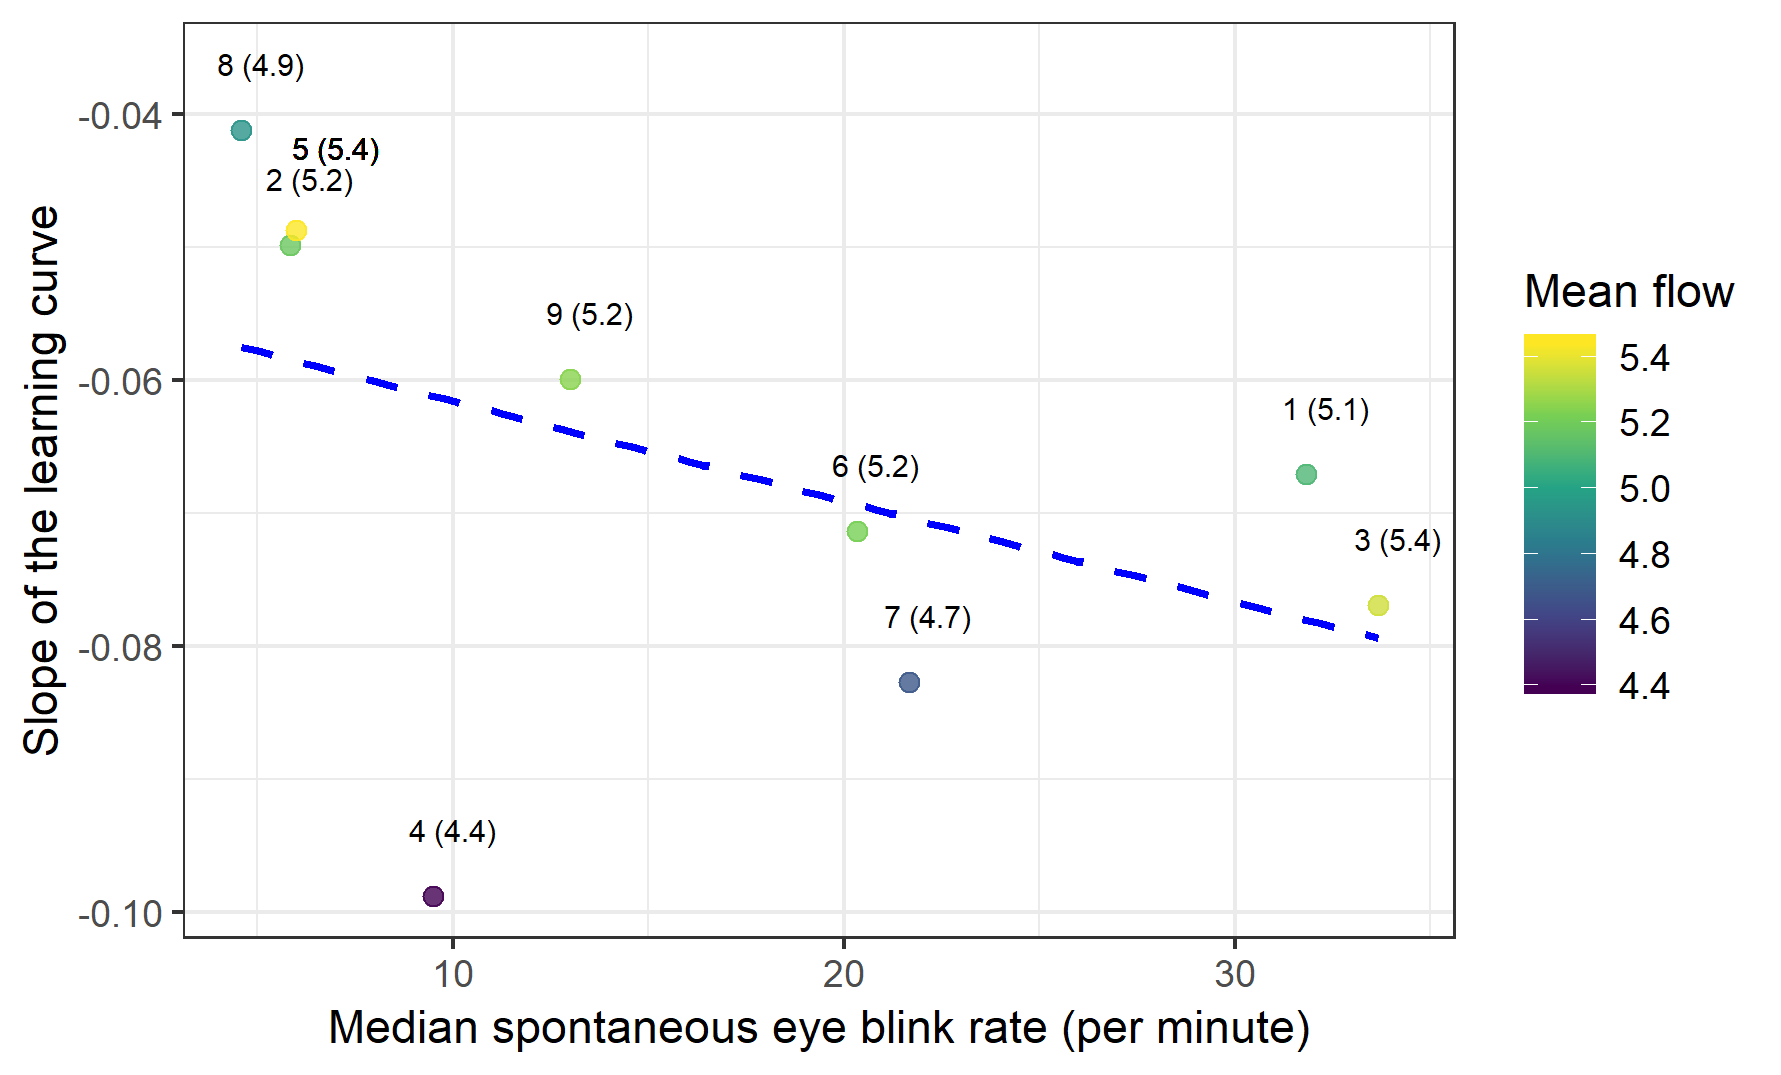
\includegraphics[width=\nicewidth]{lcurve_sbr_flowRL2}
	\caption{Participants' median spontaneous eye blink rate plotted against the slope of their learning curve, and coloured by their mean Flow scores. Linear model is depicted by the dashed line. Each point is labelled with the participant number (1..9) and exact mean Flow score (in parentheses).}
	\label{fig:EBRvLC}
\end{figure*}


% -0.859833

\begin{table}[!hb]
\centering
\caption{Outcome of simple-slopes analysis for Flow$\times$LC interaction: each row reports on the slope of LC slope at the level and value of Flow shown.}
\begin{tabular}{llllll}
\hline
Flow level & Flow & Est. & S.E. & t value & p \\
\hline
+ 1 SD & 5.40 & -1096.31 & 221.36 & -4.95 & 0.0002 \\
Mean   & 5.06 &  -683.33 & 143.15 & -4.77 & 0.0002 \\
- 1 SD & 4.73 &  -270.35 & 158.23 & -1.71 & 1.0 \\
\hline
\label{tab:simpslopes}
\end{tabular}
\end{table}

% SIMPLE SLOPES ANALYSIS
% Slope of LC when FM = 5.40 (+ 1 SD):
%      Est.   S.E. t val.    p
%  -1096.31 221.36  -4.95 0.00
% Slope of LC when FM = 5.06 (Mean):
%     Est.   S.E. t val.    p
%  -683.33 143.15  -4.77 0.00
% Slope of LC when FM = 4.73 (- 1 SD):
%     Est.   S.E. t val.    p
%  -270.35 158.23  -1.71 0.15
%
%  JOHNSON-NEYMAN INTERVAL

\subsection*{RQ2: blink rate and Flow components}
{\it session-wise within-subjects}



%%%%%%%%%%%%%%%%%%%%%%%%%%%%%%%%%%%%%%%%%%%%%%%%%%%%%%%%%%%%%%%%%%%%%%%%%%%%%%%%
%%%%%%%%%%%%%%%%%%%%%%%%%%%%%%%%%%%%%%%%%%%%%%%%%%%%%%%%%%%%%%%%%%%%%%%%%%%%%%%%
%%%%%%%%%%%%%%%%%%%%%%%%     DISCUSSION    %%%%%%%%%%%%%%%%%%%%%%%%%%%%%%%%%%%%%
\section*{Discussion}
% exploration of Flow and on-task learning (LC as opposed to pre- post)
We present a longitudinal experiment of Flow in a game-like high-speed steering task where task performance is easily parametrised and its relation to Flow and sEBR analysed. % game was fairly successful in eliciting Flow-like experiences (high baseline, score five out of seven)
To induce Flow, the game was designed to hold the balance between skill and challenge constant: the difficulty of the game continually adapted to the skill level of the participant.

...

% Without aiming to propose a new model here, we can, based on our behavioural data, consider Flow and learning
{\it A possibly useful novel way to view Flow and learning is via task complexity. Flow has been proposed to be possible in {\it any} task, complex (e.g. car driving) or simple (e.g. dish washing) \citep{Csikszentmihalyi1999}, but has also been proposed to depend on perceived task value as well as challenge--skill balance \citep{Keller2012}. One way to resolve these ideas is to consider that the individual can {\it introduce} complexity (or value) to their activity if they appear to have exhausted a task's potential to challenge them. \cite{Nakamura2002} suggest such an exploratory mechanism to explain how individuals maintain Flow in complex tasks: ``As people master challenges in an activity...to continue experiencing flow, they must identify and engage progressively more complex challenges.'' The corollary for simple tasks is that individuals {\it create} complexity, e.g. with self-defined goals \citep{Rauterberg1995}. For example, a similar state to Flow, called the Zone, has been reported for machine-gambling addicts whose pastime is in fact skill-free, but who nevertheless believe that they are skilled \citep{Schull2014}.}

{\it In other words, complex tasks have deep structure to be learned, requiring non-trivial skill acquisition for any duration of learning and thus a shallow LC (learning is slow). Importantly, the skill level does not quickly peak, such as with simpler tasks like washing the dishes, where Flow might be obtained but cannot strongly interact with learning (without self-created complexity). Learning comes into play when we consider that the same task can appear at first simple and later complex, e.g. as our experiment game.}

% Relation to previous Work on eye blink rate
\subsection*{Learning, Flow, and sEBR}
Between-subjects evidence for RQ1 suggests a clear linear trend relating sEBR and LCs (Fig.~\ref{fig:EBRvLC}): the larger the sEBR, the steeper the LC slope (or: the higher the LC intercept). The distance of data-points from the fitted model values also closely match the distribution of Flow mean scores, meaning that individuals with lowest Flow also diverge the most from the sEBR$\times$LC model. Interaction analysis then supports the idea that sEBR correlation with LC is stronger the higher the mean Flow. We thus claim that there is a genuine sEBR--LC relationship that is moderated by Flow. We cannot decide causality based on our data, but there is literature relevant to mechanisms, that can help identify future directions of inquiry.

Learning is influenced both by psychological factors (motivation, prior experience) and physio-/neurological factors. One potentially relevant factor for studying Flow and skill acquisition is the well-established relationship between attention and striatal dopamine levels \citep{Dreisbach2005}. The striatum plays a major role in decision making and reward/aversion processing, moderated by the level of tonic dopamine D2-receptors therein; the postsynaptic levels of dopamine can thus bias the entire learning process. This is illustrated for example in studies of `attentional blink' (AB) by Slagter and others \citep{Slagter2012,COLZATO2008}), which suggest a U-shaped function between tonic striatal dopamine and AB size. In other words, very high or low levels of dopamine D2-receptor density can make attention updating too rapid (distractable) or too slow (inattentive).

sEBR has been suggested as an externally-measurable index of striatal dopamine level (though caution is needed, see \cite{dang2017spontaneous}). Early work by \cite{Karson1983} linked sEBR to striatal dopamine in humans and other primates. \cite{Taylor1999} then localised to the caudate nucleus, whose normal function is implicated in classification learning \citep{Seger2005}; caudate nucleus volumetric asymmetry is implicated in inattention symptomatology \citep{Schrimsher2002}. Later work from \cite{Slagter2015} has shown that sEBRs may relate specifically to avoidance learning; others have linked dopamine levels and sEBR to perseverance, distractibility and cognitive control \citep{Muller2007,Dreisbach2005}. Finally, \cite{DeManzano2013} have shown that  predisposition to experience Flow is positively correlated with striatal dopamine D2-receptor availability (measured in PET), specifically in caudate and putamen, and stronger in right hemisphere than left.

Let us consider learning as a process whereby perception, cognition and action become attuned to task demands. In our game task, learning involves high-frequency decision making with respect to continuously updating stimuli of uniform kind (not unlike AB task, a continuous performance test designed to probe AB size \citep{Slagter2012}). In this view, the sEBR--LC relationship could be interpreted as showing that higher D2 density indexed by sEBR supports learning (LC slope). An alternative interpretation is that it reflects higher distractability in the early phases of learning (LC intercept).

The underlying mechanism could be that higher dopamine levels permit more rapid attention updating and thus more fluid response to changing task demands. This can work despite \cite{Slagter2012}'s proposed U-shaped function: because our game-task constantly maintains a level of demand slightly greater than the participants' skill. Thus, in this context, higher sEBR tends to be better, possibly because the {\it requirement} for rapid attention updating grows with the learned task skill.

Less subjective Flow was reported by those participants who deviated (positively or negatively) from this relationship. Lower Flow could be due to, e.g., misalignment of task demands and attentional updating rate, creating a more effortful experience. So the observed moderation by Flow scores of the sEBR--LC relationship could be speculated to have a basis in adjusting attention updating, in response to changing task speeds, physiologically underpinned by the nigro-striatal DA system. In other words, it may not be the case that an absolute level of striatal dopamine should predict learning, but rather an individual level relative to how each participant relates to the task (vis-\'{a}-vis gaming experience, motivation, fine motor skills, or potentially many other variables). If a participant's tonic dopamine is not at their ideal level for this task, they might nevertheless do well in the task, and yet find the experience more effortful and less fluid (than is suggested as Flow-like by wording of the FSS).


\subsection*{Limitations and Future Work}
{\it Our study had a small convenience sample because (a) the recording paradigm was extensive (around eight hours of contact time), and (b) it was to some degree an exploratory study; both implying the need to constrain datasets to tractable sizes. It is worth noting that while we recruited only 9 participants, we collected a significant amount of behavioural and physiological data for each participant over a course of two weeks and 8 recording sessions. This amounts to a particularly rich dataset allowing us to dig deep into the underpinnings of skilled high speed steering and Flow. Moreover, given the fact our experimental paradigm has not been used previously, we could not {\it a priori} easily estimate the statistical power required to discover significant effects. However, our results ended up being both strikingly {\it similar} and {\it strong} within each participant, suggesting that collecting a larger sample size would likely have {\it not} changed the pattern of the results or provided more in-depth insights. Regardless of the justifications, the sample size and method are minor limitations to be remedied in future work. Additionally, lacking experimental manipulations the study cannot make strong causal claims, which could be improved by recording separate conditions of the game task, e.g. with varied difficulty levels.}

{\it Trial-by-trial analysis is limited by the Flow self-report which only has one data point per trial. It would be more powerful to analyse {\it inside} each trial. In our data, self-reported Flow is a point model of an entire trial, for which the participant knows their score. Self-reported Flow is thus an after-the-fact report, and could be criticized for not capturing the in-the-moment {\it experience of Flow}, which might fluctuate greatly during a trial. Analysing the fluctuation of Flow-experience requires us to model individual actions and/or their outcomes, and sample Flow during performance. This is a difficult challenge, because paying attention to one's phenomenal state might easily disrupt the very processes sustaining that state, especially for Flow which is unreflective by definition. Future work should aim to model the conditions of Flow ({\sf C1--3}) in real-time, while simultaneously recording participant physiology, to uncover in greater detail the relationships involved. The existing dataset will be used for this purpose, in a pending report on the biosignals recorded with high temporal resolution, primarily electro-dermal activity.}

To further explore the possible role of striatal dopamine, it would be interesting to experimentally manipulate the game to adjust the distance between obstacles, thus altering the attention-updating rate required to navigate without collisions (motor precision variation can be minimised by a suitably long training period). This manipulation could be varied in response to measurements of sEBR (which can be automated, e.g. by using electro-oculography \citep{toivanen2014}), to systematically investigate whether sEBR holds explanatory power with respect to individual variability in learning.


\subsection*{Conclusion}

% We report evidence that the LC across sessions is predicted by participants' spontaneous blink rate.
We report evidence that slope of the learning curve (total play time about 2 h, distributed over two weeks) is predicted by the participants' spontaneous blink rate, moderated by global Flow. This relationship potentially indicates a role for striatal dopamine in learning the visuomotor steering task, which may interact with the experience of Flow.

Understanding how perceptual-cognitive and motor processes underlying performance give rise to phenomenological experiences, such as Flow, and how the phenomenal experiences relate to performance on the other is an important topic for understanding human motivation and performance. This study contributes to this goal and we hope will inspire more inquiry into the dynamics of the Flow experience in different stages of learning a skill.


\subsection*{Context}
The three senior authors conceived and guided the work. BC (the lead author) has studied computer gameplay from the perspective of performance, psychophysiology and emotional experiences. OL (the last author) has studied visuomotor skill in the domain of high-speed steering, and developed the game with JV to extend the research into the direction of Flow research. JP (the second author) has studied emotions and decision-making in games of skill and chance, and written on the similarities and differences between the Zone and Flow phenomena. Because these authors share a keen interest in understanding the development of expertise and the phenomenon of Flow, it was decided to join forces and put together a team of researchers to develop the present experiment on the basis of the `Flow-inducing' high-speed steering game designed earlier. The other authors (all more junior graduate students) were recruited to work as part of their studies. This experiment is part of a larger effort to initiate a line of research into the neurocognitive processes underlying Flow and expert performance, combining experimental, psychophysiological and computational methods.


%%%%%%%%%%%%%%%%%%%%%%%%%%%%%%%%%%%%%%%%%%%%%%%%%%%%%%%%%%%%%%%%%%%%%%%%%%%%%%%%
%%%%%%%%%%%%%%%%%%%%%%%%%%%%%%%%%%%%%%%%%%%%%%%%%%%%%%%%%%%%%%%%%%%%%%%%%%%%%%%%
%%%%%%%%%%%%%%%%%%%%% POST-HOC MATERIAL OF VITAL IMPORTANCE %%%%%%%%%%%%%%%%%%%%
\bibliography{cleanbib/CogCarFlow_bib}


\section*{Acknowledgements}


\section*{Author contributions statement}
% please edit as appropriate
OL, JP and BUC conceived the study.
OL and JV designed the gameplay.
JV implemented the game.
BUC and TT designed and implemented the data collection.
NL, TT, PP, RF, VPI, and JP translated the FSS.
All authors participated in decisions on the experiment specifications.
RF, VPI, NL, PP, and TT conducted the experiment.
BUC, VPI, TT, RF, PP, NL, JP, and OL analysed and interpreted the results.
BUC, JP and OL drafted the paper.
All authors participated in writing and reviewing, and approved the manuscript.


\end{document}
